%%%%%%%%%%%%%%%%%%%%%%%
% Syracuse Conference Talk
%%%%%%%%%%%%%%%%%%%%%%%

% Title Slide
\begin{frame}[plain]
	\maketitle
\end{frame}



% Quote
{\setbeamertemplate{background canvas}{
\tikz[remember picture,overlay]
	\node[opacity=0.3] at (current page.center) {
	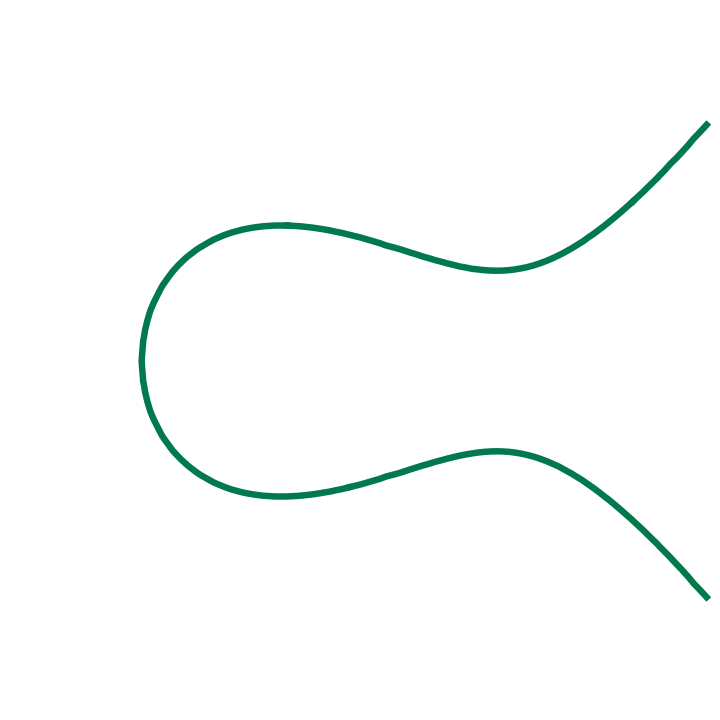
\includegraphics[width=\paperwidth,
	height=\paperheight]{images/curve.png}};} 
\begin{frame}[plain]
	\begin{minipage}{0.2\textwidth}
 	\begin{figure}[h]
	\centering
	\fbox{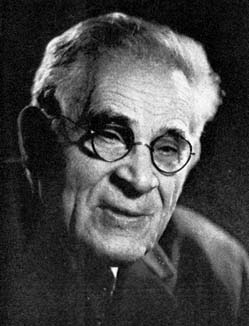
\includegraphics[width=1\textwidth]{images/mordell.jpg}} \par
	{\small 1888--1972}
	\end{figure}
	\end{minipage}%
	\begin{minipage}{0.8\textwidth}
	\begin{center}
	{\itshape ``Mathematicians have been familiar with very few questions for so long a period with so little accomplished in the way of general results, as that of finding the rational [points on elliptic curves].''} \\
	 \phantom{x}\hfill-- L.J. Mordell, 1922
	\end{center}
 	\end{minipage}
\end{frame}
}



% Mordell Theorem
\begin{frame}[plain]
	\begin{thm}[Mordell, 1922]
	Let $E/\Q$ be an elliptic curve. Then the group of rational points on $E$, denoted $E(Q)$ is a finitely generated abelian group. In particular, 
		\[
		E(\Q) \cong \Z^r \oplus E(\Q)_\tors,
		\]
	where $r \geq 0$ is the rank and $E(\Q)_\tors$ is the set of points with finite order. 
	\end{thm}
	\begin{figure}[h]
	\captionsetup{labelformat=empty}
	\centering
	\fbox{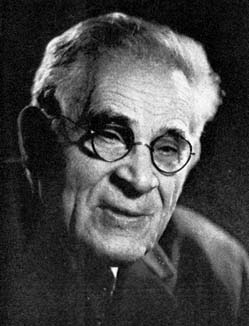
\includegraphics[width=0.20\textwidth]{images/mordell.jpg}}
	\caption{Louis J. Mordell \\ 1888--1972}
	\end{figure}
\end{frame}


% Mordell - Weil - Neron
\begin{frame}[plain]
	\begin{thm}[Mordell-Weil-N\'eron, 1952]
	Let $K$ be a field that is finitely generated over its prime field and $A/K$ be an abelian variety. Then the group of $K$-rational points on $A$, denoted $A(K)$, is a finitely generated abelian group. In particular,
		\[
		A(K) \cong \Z^{r_{A/K}} \oplus A(K)_\tors
		\]
	\end{thm}
	\begin{figure}[h]
	\centering
	\begin{subfigure}{0.3\textwidth}
	\captionsetup{labelformat=empty}
	\centering
	\fbox{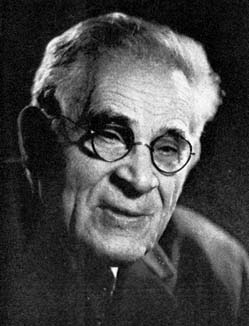
\includegraphics[width=0.8\textwidth]{images/mordell.jpg}}
	\caption{\hspace{0.5cm}Louis J. Mordell \\ \hspace{0.8cm}1888--1972}
	\end{subfigure}
	%
	\begin{subfigure}{0.3\textwidth}
	\captionsetup{labelformat=empty}
	\centering
	\fbox{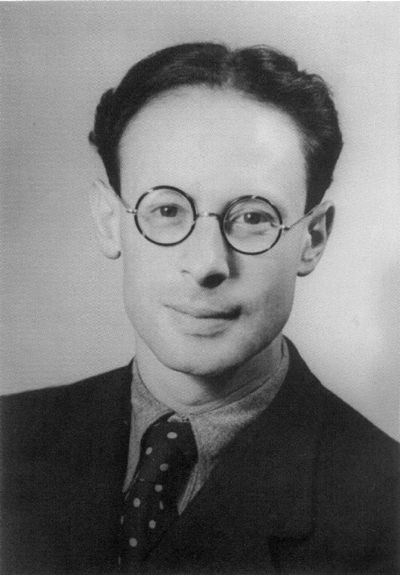
\includegraphics[width=0.74\textwidth]{images/weil.jpg}}
	\caption{Andr\'e Weil \\ 1906--1998}
	\end{subfigure}
	%
	\begin{subfigure}{0.3\textwidth}
	\captionsetup{labelformat=empty}
	\centering
	\fbox{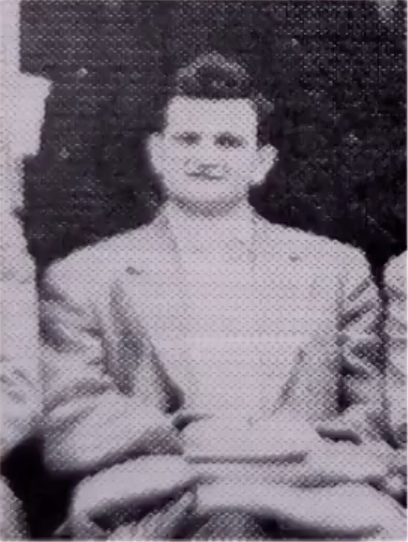
\includegraphics[width=0.81\textwidth]{images/neron.png}}
	\caption{\hspace{0.6cm}Andr\'e N\'eron \\ \hspace{0.75cm}1922--1985}
	\end{subfigure}
	\end{figure}
\end{frame}


% E(K) Torsion Structure
\begin{frame}[plain]
\frametitle{\textcolor{white}{Structure of the Torsion Subgroup}}
	\[
	\begin{split}
	E(K)_{\text{tors}} &\cong\; \qfrac{\Z}{m\Z} \oplus \qfrac{\Z}{mn\Z} \\[0.5cm]
	E[n] &\cong\; \qfrac{\Z}{n\Z} \oplus \qfrac{\Z}{n\Z}
	\end{split}
	\]
\end{frame}


% Mazur
\begin{frame}[plain]
\begin{thm}[Levi-Ogg Conjecture; Mazur, 1977]
If $E/\Q$ is a rational elliptic curve, then $E(\Q)_\tors$ is isomorphic to precisely one of the following:
	\[
	\begin{cases}
	\Z/n\Z, & n=1,2,\ldots,10,12 \\
	\Z/2\Z \oplus \Z/2n\Z, & n=1,\ldots,4
	\end{cases}
	\]
Moreover, each possibility occurs infinitely often.
\end{thm}
	\begin{figure}[h]
	\centering
	\begin{subfigure}{0.3\textwidth}
	\captionsetup{labelformat=empty}
	\centering
	\fbox{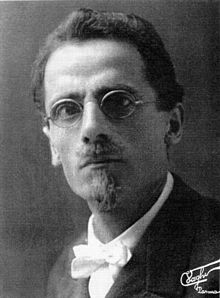
\includegraphics[width=0.72\textwidth]{images/levi.jpg}}
	\caption{\hspace{0.5cm}Beppo Levi \\ \hspace{0.8cm}1875--1961}
	\end{subfigure}
	%
	\begin{subfigure}{0.3\textwidth}
	\captionsetup{labelformat=empty}
	\centering
	\fbox{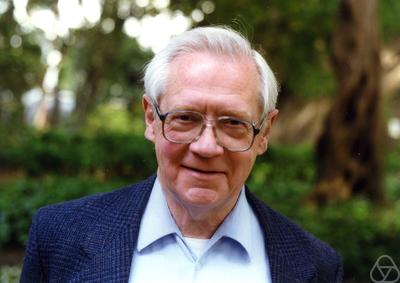
\includegraphics[width=\textwidth]{images/ogg.jpg}}
	\caption{Andrew Ogg \\ 1934 --}
	\end{subfigure} \quad
	%
	\begin{subfigure}{0.3\textwidth}
	\captionsetup{labelformat=empty}
	\centering
	\fbox{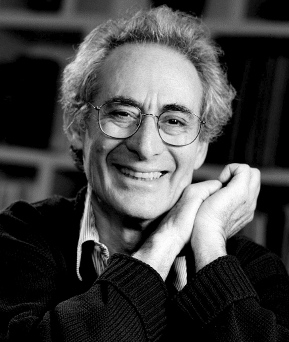
\includegraphics[width=0.82\textwidth]{images/mazur.jpg}}
	\caption{\hspace{0.6cm}Barry Mazur \\ \hspace{0.75cm}1937 --}
	\end{subfigure}
	\end{figure}
\end{frame}


% Question
\begin{frame}[plain]
	\begin{ques}
	What finitely generated abelian groups arise from abelian varieties over global fields? 
	\end{ques}	
\end{frame}


% Question
\begin{frame}[plain]
	\begin{ques}
	What torsion subgroups arise for elliptic curves $E/K$, where $K$ is a number field of degree $d$? 
	\end{ques}	
\end{frame}


% WLOG
\begin{frame}[plain]
\ctext{With massive loss of generality, let $d=2$.}
\end{frame}


% Quadratic
\begin{frame}[plain]
\begin{thm}[Kenku, Momose, 1988; Kamienny, 1992]
 Let $K/\Q$ be a quadratic number field and $E/K$ be an elliptic curve. Then $E(K)_\tors$ is isomorphic to precisely one of the following:
 	\[
	\begin{cases}
	\Z/n\Z, & n=1,2,\ldots,16,18 \\
	\Z/2\Z \oplus \Z/2n\Z, & n=1,\ldots,6 \\
	\Z/3\Z \oplus \Z/3n\Z, & n=1,2 \\
	\Z/4\Z \oplus \Z/4\Z
	\end{cases}
	\]
Moreover, each possibility occurs infinitely often. 
\end{thm}
	\begin{figure}[h]
	\centering
	\begin{subfigure}{0.3\textwidth}
	\captionsetup{labelformat=empty}
	\centering
	\fbox{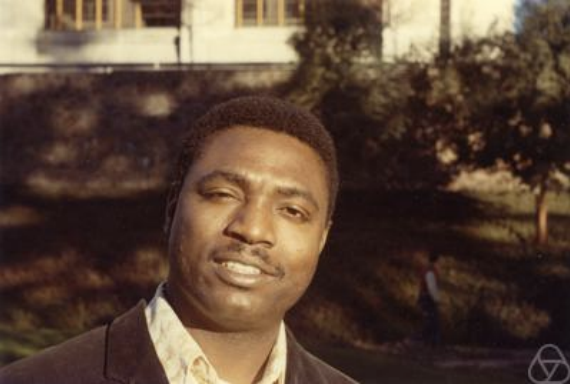
\includegraphics[width=0.94\textwidth]{images/kenku.png}}
	\caption{Monsur Kenku}
	\end{subfigure} \quad
	%
	\begin{subfigure}{0.3\textwidth}
	\captionsetup{labelformat=empty}
	\centering
	\fbox{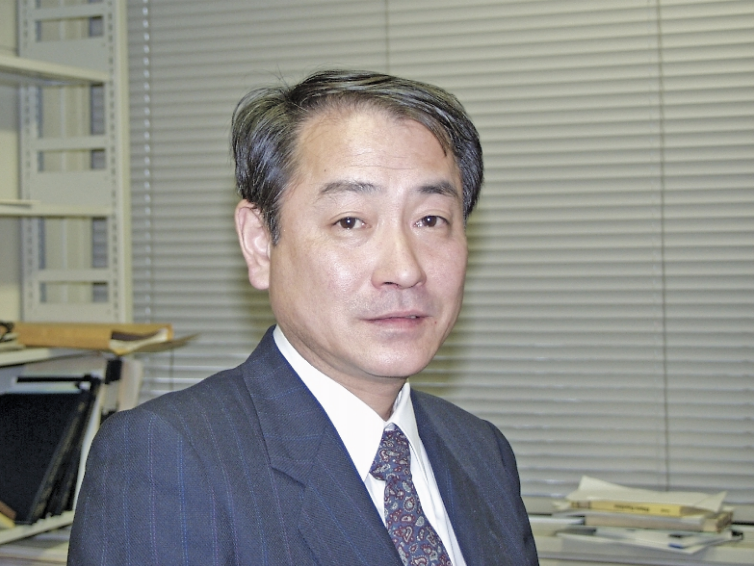
\includegraphics[width=0.85\textwidth]{images/momose.png}}
	\caption{Fumiyuki Momose}
	\end{subfigure}
	%
	\begin{subfigure}{0.3\textwidth}
	\captionsetup{labelformat=empty}
	\centering
	\fbox{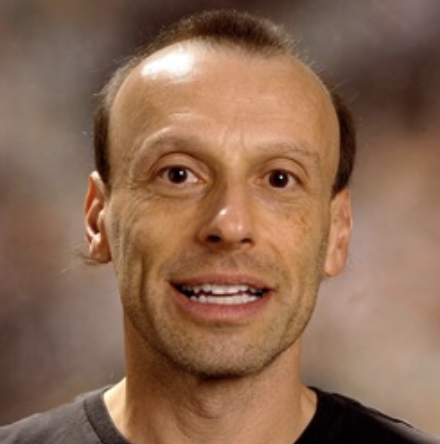
\includegraphics[width=0.65\textwidth]{images/kamienny.png}}
	\caption{Sheldon Kamienny}
	\end{subfigure}
	\end{figure}
\end{frame}


% Cubic
\begin{frame}[plain]
\begin{thm}[Jeon,Kim,Schweizer, 2004; Etropolski-Morrow-Zureick Brown; Derickx, 2016]
Let $K/\Q$ be a cubic number field and $E/K$ be an elliptic curve. Then $E(K)_\tors$ is isomorphic to precisely one of the following:
	\[
	\begin{cases}
	\Z/n\Z & n=1,2,\ldots,16,18,20,21 \\
	\Z/2n\Z & n=1,\ldots,7
	\end{cases}
	\]
Each of these possibilities occurs infinitely many times except $\Z/21\Z$.
\end{thm}
	\begin{figure}[h]
	\centering
	\begin{subfigure}{0.10\textwidth}
	\captionsetup{labelformat=empty}
	\centering
	\fbox{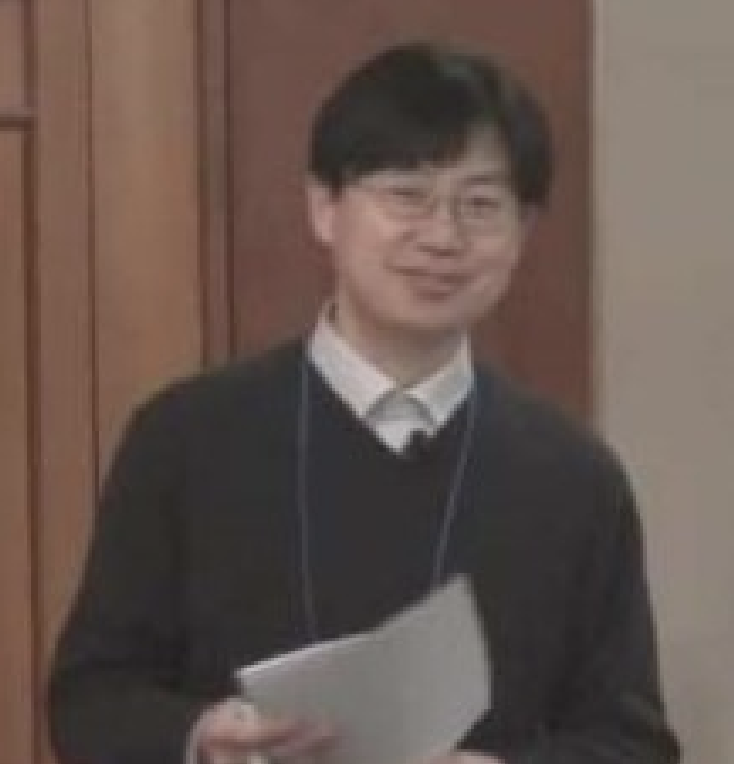
\includegraphics[width=1.2\textwidth]{images/jeon.png}}
	\caption{\hspace{0.2cm}\scriptsize{Jeon}}
	\end{subfigure} \quad\quad
	%
	\begin{subfigure}{0.10\textwidth}
	\captionsetup{labelformat=empty}
	\centering
	\fbox{
\includegraphics[width=1.2\textwidth]{images/kim.jpg}}
	\caption{\hspace{0.3cm}\scriptsize{Kim}}
	\end{subfigure} \quad\quad
	%
	\begin{subfigure}{0.10\textwidth}
	\captionsetup{labelformat=empty}
	\centering
	\fbox{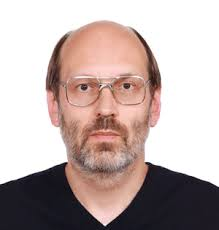
\includegraphics[width=1.2\textwidth]{images/schweizer.jpeg}}
	\caption{\hspace{0.1cm}\scriptsize{Schweizer}}
	\end{subfigure} \\
	%
	\hfill
	\begin{subfigure}{0.12\textwidth}
	\captionsetup{labelformat=empty}
	\centering
	\fbox{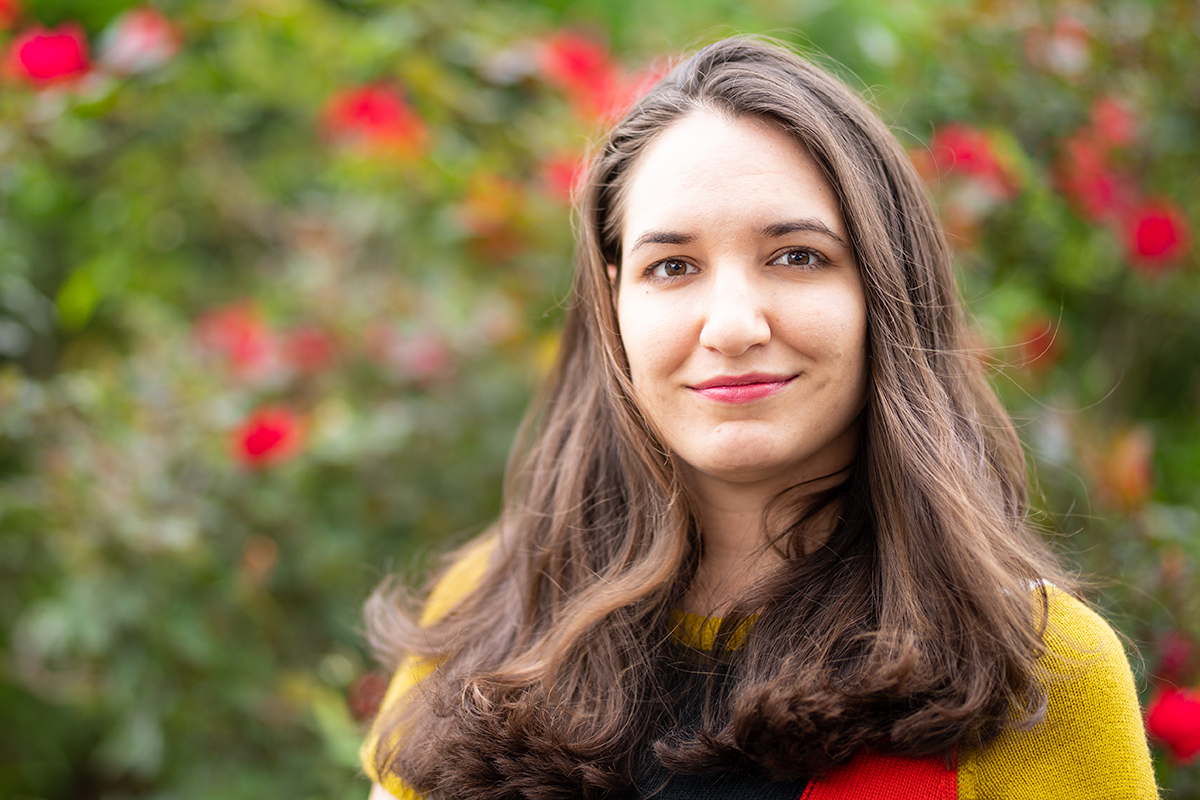
\includegraphics[width=1.5\textwidth]{images/etropolski.jpg}}
	\caption{\;\;\;\;\scriptsize{Etropolski}}
	\end{subfigure} \hfill
	%
	\begin{subfigure}{0.10\textwidth}
	\captionsetup{labelformat=empty}
	\centering
	\fbox{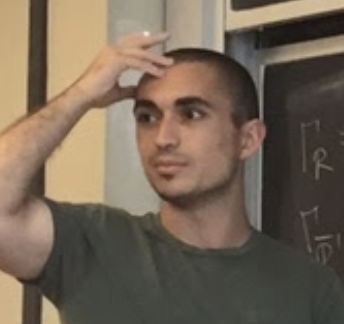
\includegraphics[width=1.5\textwidth]{images/morrow.png}}
	\caption{\;\;\;\scriptsize{Morrow}}
	\end{subfigure} \hfill
	%
	\begin{subfigure}{0.10\textwidth}
	\captionsetup{labelformat=empty}
	\centering
	\fbox{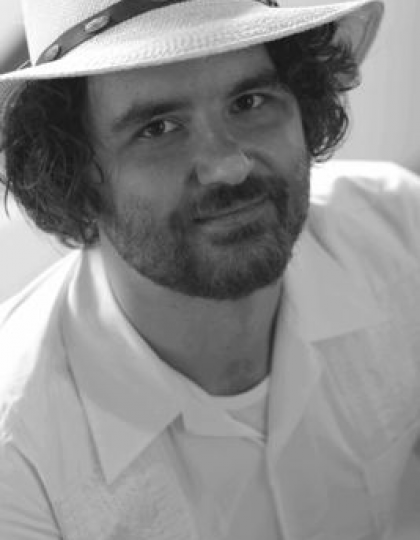
\includegraphics[width=1.15\textwidth]{images/zbrown.png}}
	\caption{\;\;\scriptsize{Z-B.}}
	\end{subfigure} \hfill
	%
	\begin{subfigure}{0.10\textwidth}
	\captionsetup{labelformat=empty}
	\centering
	\fbox{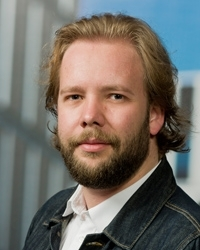
\includegraphics[width=1.2\textwidth]{images/derickx.jpg}}
	\caption{\;\;\scriptsize{Derickx}}
	\end{subfigure} \hfill \phantom{I}
	\end{figure}
\end{frame}


% Quartic
\begin{frame}[plain]
\begin{thm}[Jeon, Kim, Park, 2006]
Let $K/\Q$ be a quartic number field and $E/K$ be an elliptic curve. Then the possible torsion subgroups $E(K)_\tors$ appearing infinitely often are precisely:
	\[
	\begin{cases}
	\Z/n\Z, & n=1,2,\ldots,18,20,21,22 \\
	\Z/2\Z \oplus \Z/2n\Z, & n=1,\ldots,9 \\
	\Z/3\Z \oplus \Z/3n\Z, & n=1,2,3 \\
	\Z/4\Z \oplus \Z/4n\Z, & n=1,2 \\
	\Z/5\Z \oplus \Z/5\Z \\
	\Z/6\Z \oplus \Z/6\Z
	\end{cases}
	\]
\end{thm}
	\begin{figure}[h]
	\centering
	\begin{subfigure}{0.3\textwidth}
	\captionsetup{labelformat=empty}
	\centering
	\fbox{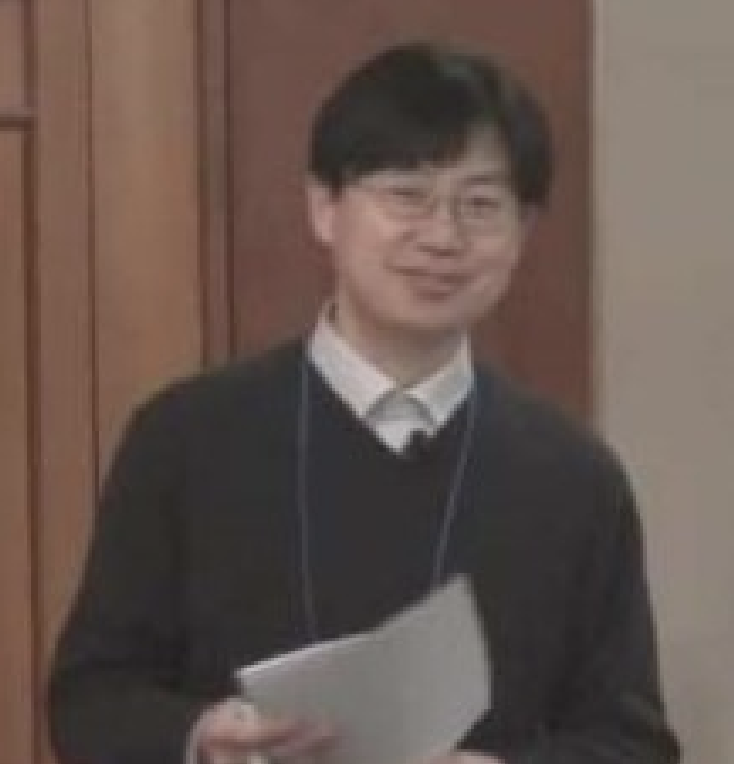
\includegraphics[width=0.60\textwidth]{images/jeon.png}}
	\caption{\hspace{0.1cm}Daeyeol Jeon}
	\end{subfigure}
	%
	\begin{subfigure}{0.3\textwidth}
	\captionsetup{labelformat=empty}
	\centering
	\fbox{
\includegraphics[width=0.63\textwidth]{images/kim.jpg}}
	\caption{Chang Kim}
	\end{subfigure}
	%
	\begin{subfigure}{0.3\textwidth}
	\captionsetup{labelformat=empty}
	\centering
	\fbox{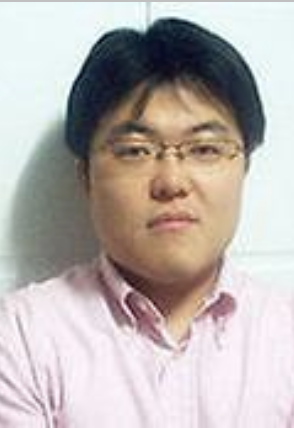
\includegraphics[width=0.45\textwidth]{images/park.png}}
	\caption{\hspace{0cm}Eui-Sung Park}
	\end{subfigure}
	\end{figure}
\end{frame}


% Quintic
\begin{frame}[plain]
\begin{thm}[Derickx, Sutherland, 2016]
Let $K/\Q$ be a quintic number field and $E/K$ be an elliptic curve. Then the possible torsion subgroups $E(K)_\tors$ appearing infinitely often are precisely:
	\[
	\begin{cases}
	\Z/n\Z, & n=1,\ldots,22,24,25 \\
	\Z/2\Z \oplus \Z/2n\Z, & n=1,\ldots,8
	\end{cases}
	\]
\end{thm}
	\begin{figure}[h]
	\centering
	\begin{subfigure}{0.3\textwidth}
	\captionsetup{labelformat=empty}
	\centering
	\fbox{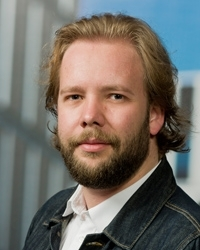
\includegraphics[width=0.72\textwidth]{images/derickx.jpg}}
	\caption{\hspace{0.1cm}Maarten Derickx}
	\end{subfigure}
	%
	\begin{subfigure}{0.3\textwidth}
	\captionsetup{labelformat=empty}
	\centering
	\fbox{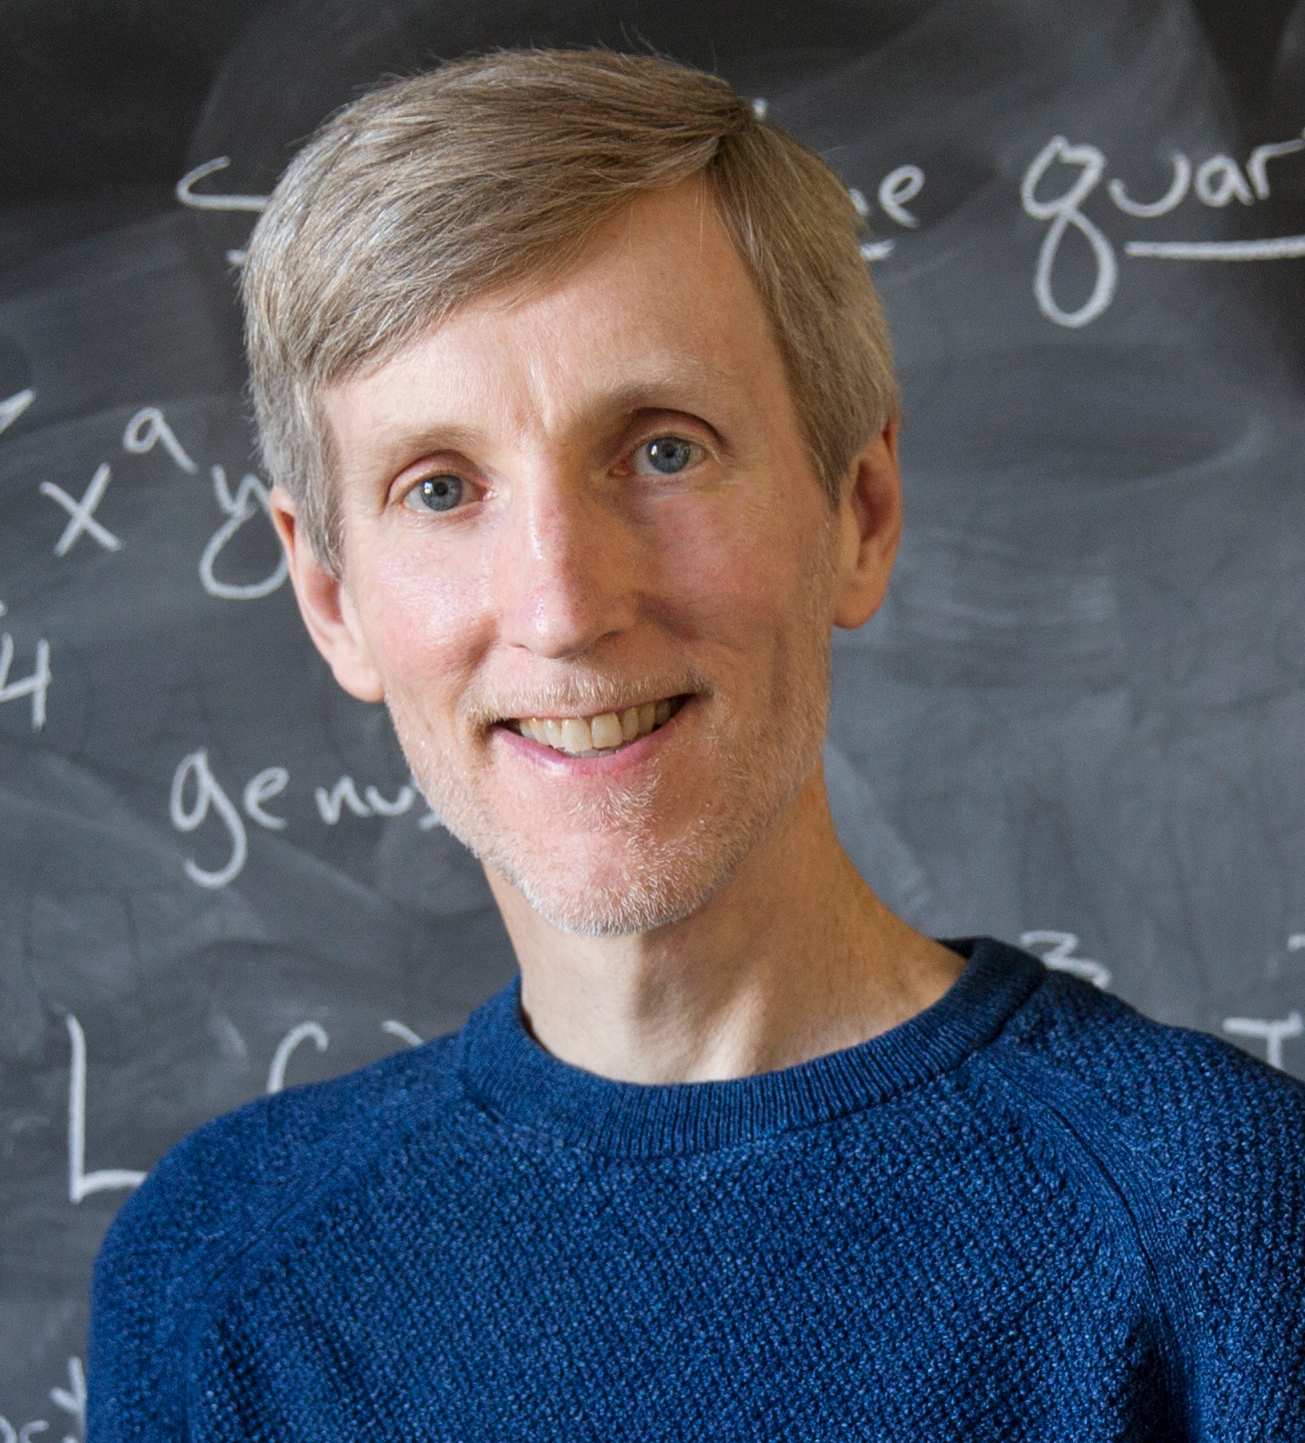
\includegraphics[width=0.82\textwidth]{images/sutherland.jpg}}
	\caption{Drew Sutherland}
	\end{subfigure}
	\end{figure}
\end{frame}


% Sextic
\begin{frame}[plain]
\begin{thm}[Derickx, Sutherland, 2016]
Let $K/\Q$ be a sextic number field and $E/K$ be an elliptic curve. Then the possible torsion subgroups $E(K)_\tors$ appearing infinitely often are precisely:
	\[
	\begin{cases}
	\Z/n\Z, &  n=1,\ldots,30; n \neq 23,25,29 \\
	\Z/2\Z \oplus \Z/2n\Z, & n=1,\ldots,10 \\
	\Z/3\Z \oplus \Z/3n\Z, & n=1,\ldots,4 \\
	\Z/4\Z \oplus \Z/4n\Z, & n=1,2 \\
	\Z/6\Z \oplus \Z/6\Z 
	\end{cases}
	\]
\end{thm}
	\begin{figure}[h]
	\centering
	\begin{subfigure}{0.3\textwidth}
	\captionsetup{labelformat=empty}
	\centering
	\fbox{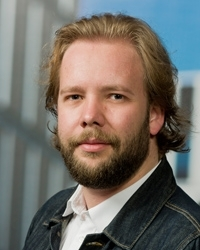
\includegraphics[width=0.72\textwidth]{images/derickx.jpg}}
	\caption{\hspace{0.1cm}Maarten Derickx}
	\end{subfigure}
	%
	\begin{subfigure}{0.3\textwidth}
	\captionsetup{labelformat=empty}
	\centering
	\fbox{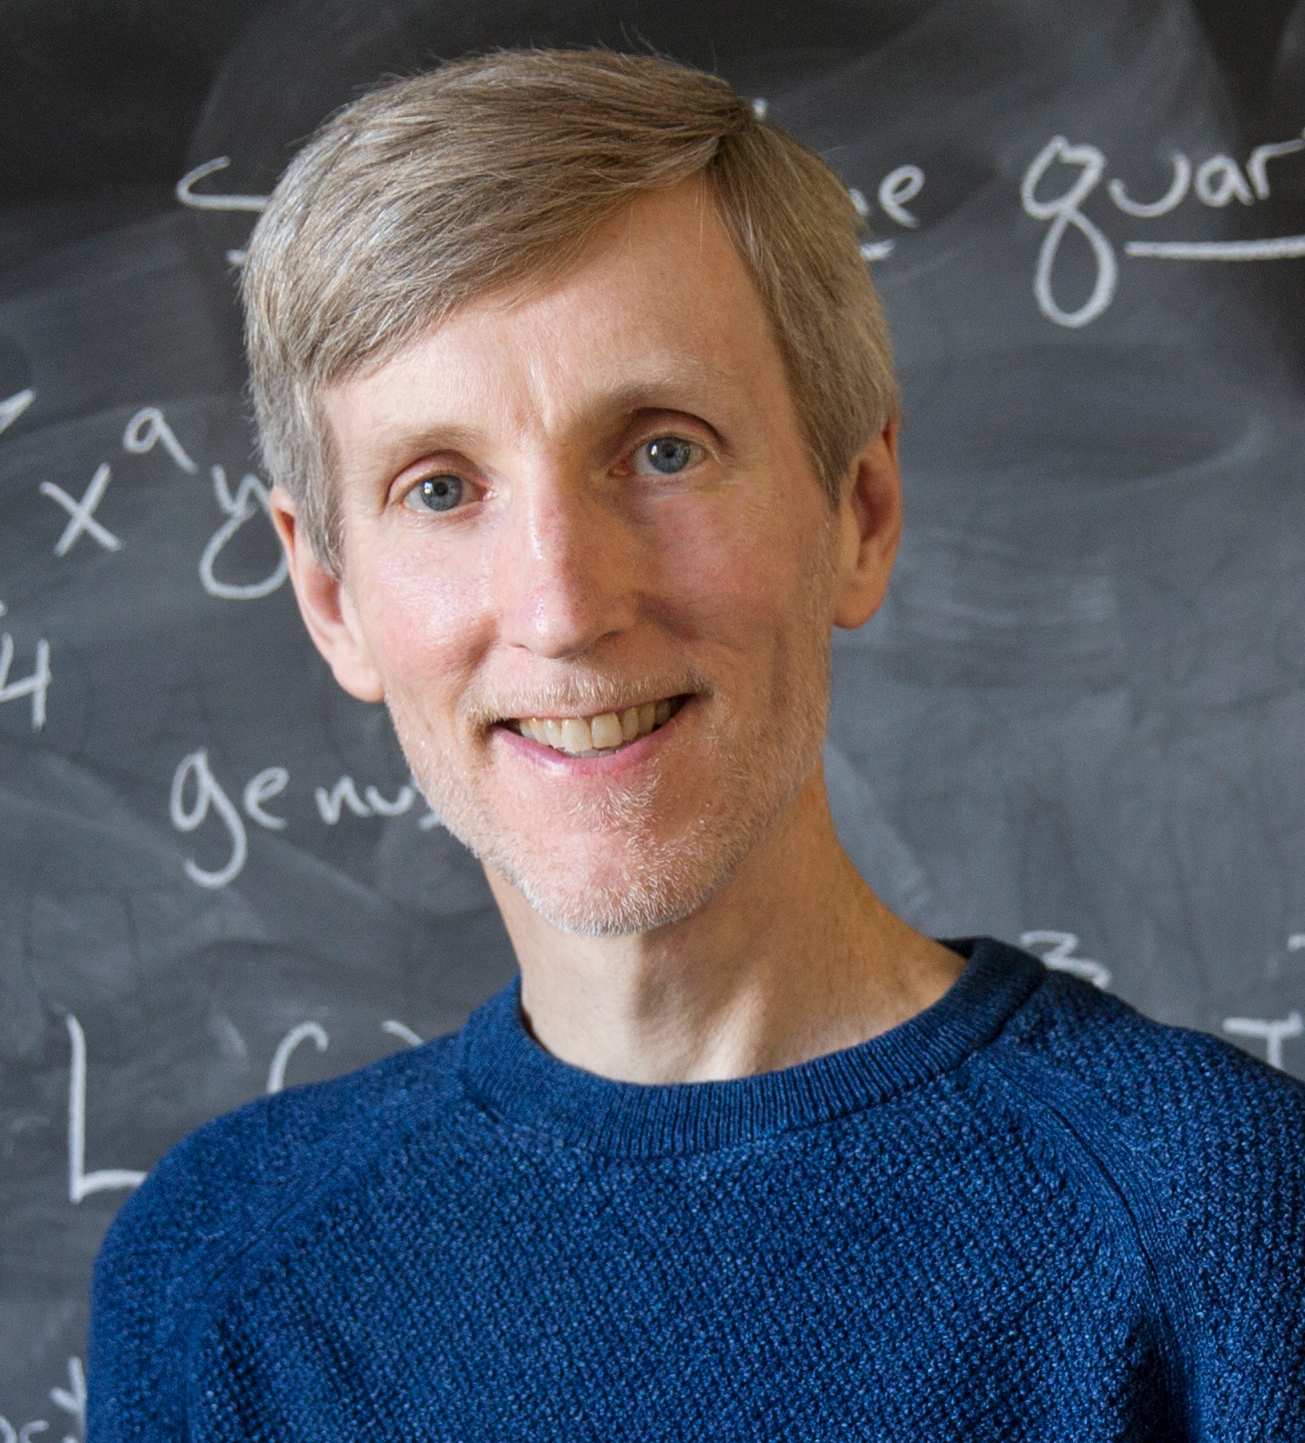
\includegraphics[width=0.82\textwidth]{images/sutherland.jpg}}
	\caption{Drew Sutherland}
	\end{subfigure}
	\end{figure}
\end{frame}


% CM Curves
\begin{frame}[plain]
	\begin{thm}[Clark, Corn, Rice, Stankewicz; 2013]
	Let $K$ be a number field of degree $d=1,2,\ldots,13$ and $E/K$ be an elliptic curve with CM. Then all possible torsion subgroups are given, and an algorithm to compute the list.
	\end{thm} 
	\begin{figure}[h]
	\centering
	\begin{subfigure}{0.23\textwidth}
	\captionsetup{labelformat=empty}
	\centering
	\fbox{
\includegraphics[width=0.75\textwidth]{images/clark.jpg}}
	\caption{Pete Clark}
	\end{subfigure}
	%
	\begin{subfigure}{0.23\textwidth}
	\captionsetup{labelformat=empty}
	\centering
	\fbox{
\includegraphics[width=0.83\textwidth]{images/corn.jpg}}
	\caption{Patrick Corn}
	\end{subfigure}
	%
	\begin{subfigure}{0.23\textwidth}
	\captionsetup{labelformat=empty}
	\centering
	\fbox{
\includegraphics[width=1.0\textwidth]{images/rice.png}}
	\caption{Alex Rice}
	\end{subfigure}
	%
	\begin{subfigure}{0.25\textwidth}
	\captionsetup{labelformat=empty}
	\centering
	\fbox{
\includegraphics[width=0.65\textwidth]{images/stankewicz.png}}
	\caption{James Stankewicz}
	\end{subfigure}
	\end{figure}
\end{frame}


% Rational
\begin{frame}[plain]
\ctext{What if you restrict to rational elliptic curves?}
\end{frame}


% Isogeny
\begin{frame}[plain]
	\begin{dfn}[Isogeny]
	Let $E_1,E_2$ be elliptic curves. An isogeny from $E_1$ to $E_2$ is a morphism $\phi: E_1 \to E_2$ with $\phi(\mathcal{O})=\mathcal{O}$. If $|\ker \phi|=n$, we say $\phi$ is an $n$-isogeny. 
	\end{dfn} \pause

	\begin{thm}[Fricke, Kenku, Klein, Kubert, Ligozat, Mazur, Ogg, et al.]
	If $E/\Q$ has an $n$-isogeny over $\Q$, then 
		\[
		n \in \{1,2,\ldots,19,21,25,27,37,43,67,163\}. 
		\]
	If $E$ does not have CM, then $n \leq 18$ or $n \in \{21,25,37\}$. 
	\end{thm}
\end{frame}


% 2-adic
\begin{frame}[plain]
\begin{thm}[Rouse,Zureick-Brown, 2015]
Let $E/\Q$ be a rational elliptic curve without CM. Then the index of $\rho_{E,2^\infty}(\Gal(\overline{\Q}/Q))$ divides 64 or 96, and all such indices occur. Furthermore, the image of $\rho_{E,2^\infty}(\Gal(\overline{\Q}/\Q))$ is the inverse image in $\GL_2(\Z_2)$ of the image of $\rho_{E,32}(\Gal(\overline{\Q}/\Q))$.
\end{thm}
	\begin{figure}[h]
	\centering
	\begin{subfigure}{0.3\textwidth}
	\captionsetup{labelformat=empty}
	\centering
	\fbox{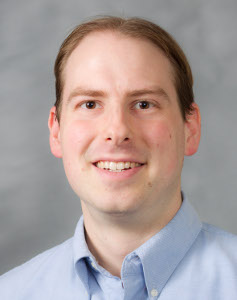
\includegraphics[width=0.70\textwidth]{images/rouse.jpg}}
	\caption{Jeremy Rouse}
	\end{subfigure}
	%
	\begin{subfigure}{0.3\textwidth}
	\captionsetup{labelformat=empty}
	\centering
	\fbox{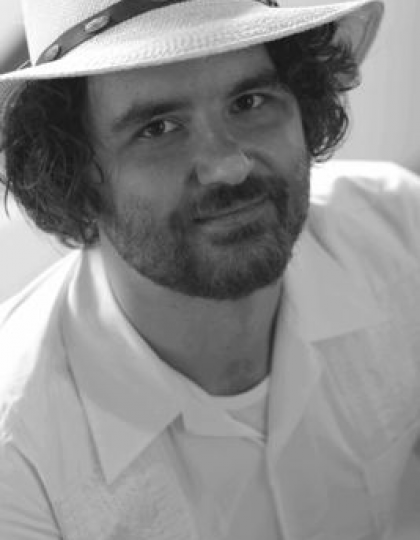
\includegraphics[width=0.69\textwidth]{images/zbrown.png}}
	\caption{David Zureick-Brown}
	\end{subfigure}
	\end{figure}
\begin{rem}
They also enumerate all 1,208 possibilities and find their rational points. 
\end{rem}
\end{frame}


% Zwyina
\begin{frame}[plain]
\begin{thm}[Sutherland, Zywina, 2016]
Up to conjugacy, there are 248 open subgroups of $\GL_2(\hat{\Z})$ of prime power level satisfying $-I \in G$ and $\det G= \hat{\Z}^\times$ for which $X_G$ has infinitely many rational points. Of these 248 groups, there are 220 of genus 0 and 28 of genus 1. 
\end{thm}
	\begin{figure}[h]
	\centering
	\begin{subfigure}{0.3\textwidth}
	\captionsetup{labelformat=empty}
	\centering
	\fbox{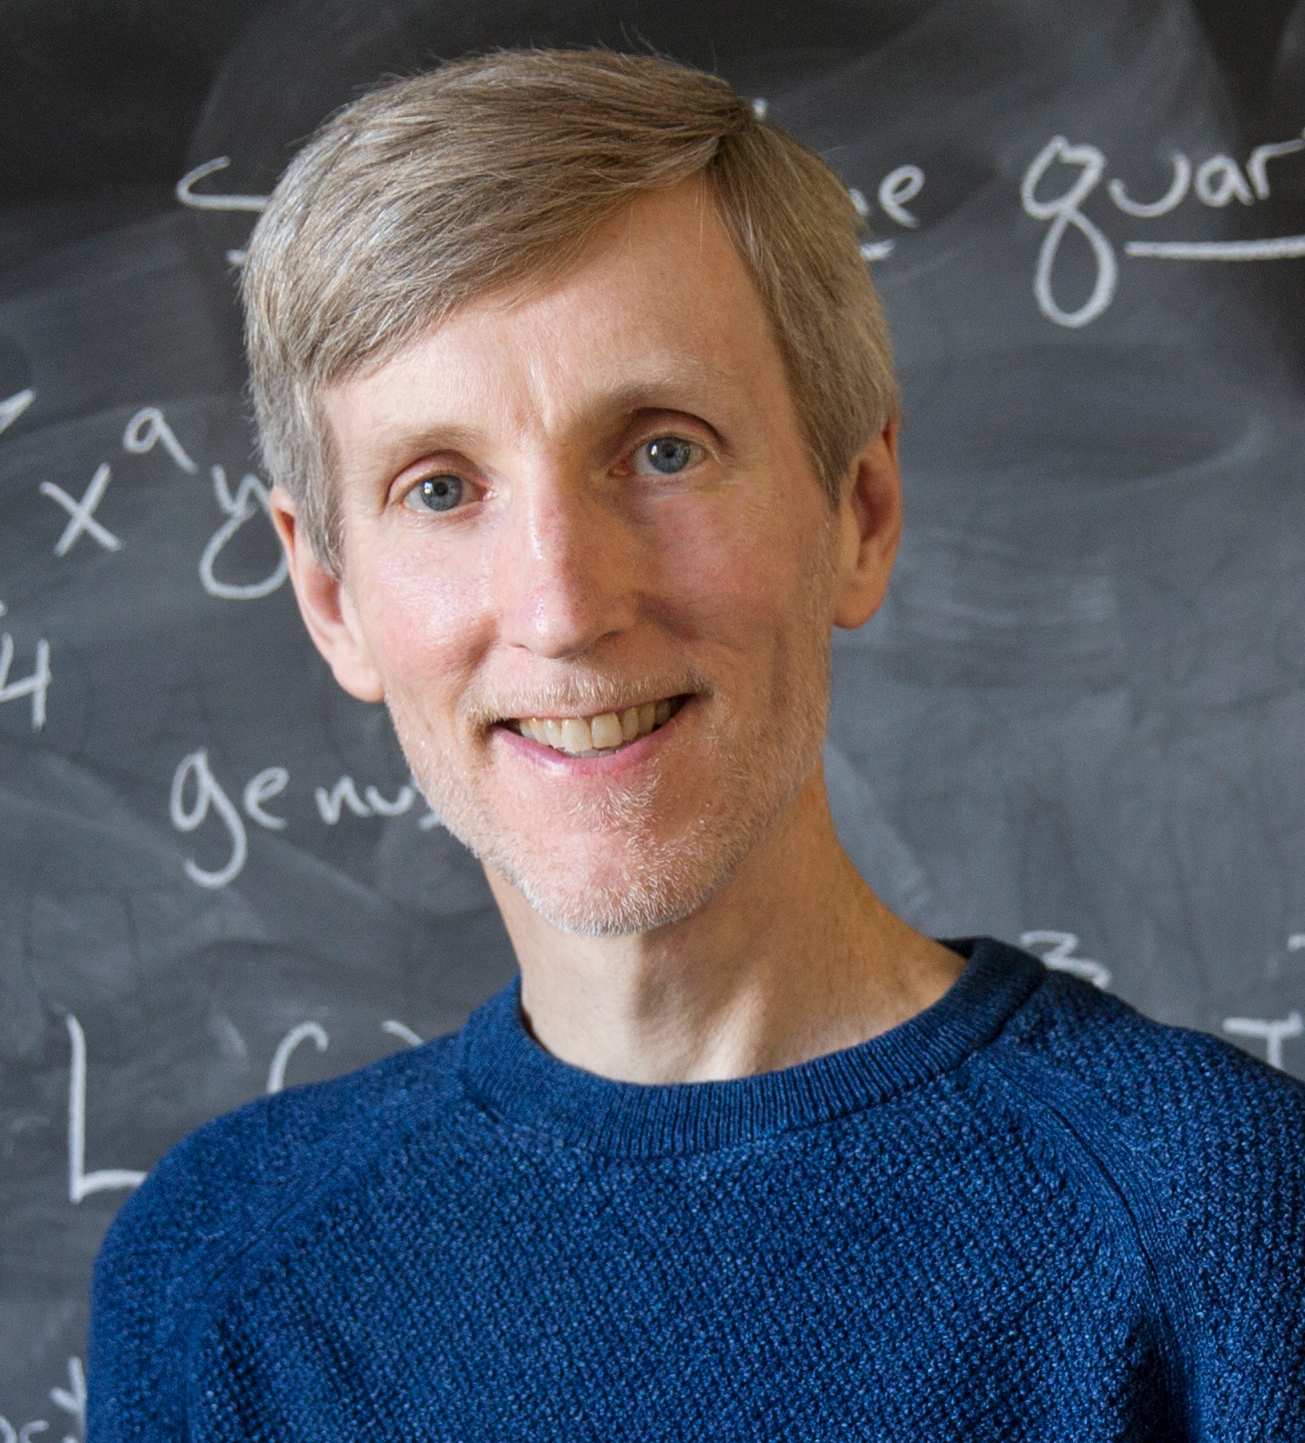
\includegraphics[width=0.82\textwidth]{images/sutherland.jpg}}
	\caption{Drew Sutherland}
	\end{subfigure}
	%
	\begin{subfigure}{0.3\textwidth}
	\captionsetup{labelformat=empty}
	\centering
	\fbox{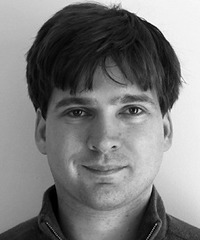
\includegraphics[width=0.77\textwidth]{images/zwyina.jpg}}
	\caption{\hspace{0.1cm}David Zywina}
	\end{subfigure}
	\end{figure}
\end{frame}


% Notation
\begin{frame}[plain]
\ctext{A bit of notation}
\end{frame}


% Notation
\begin{frame}[plain]
	\[
	\Phi_\Q(d):=\{\text{Set of Iso. Classes of } E(K)_{\text{tors}} \colon E_\Q(K), [K \colon \Q]=d\}
	\] \pause
	
	\[
	S_\Q(d):=\{ p \text{ prime} \colon \exists\ E_\Q(K), p \text{ divides } |E_\Q(K)|_{\text{tors}}, [K \colon \Q] \leq d \}
	\] 
\end{frame}


% Base Extension
\begin{frame}[plain]
\ctext{What happens to torsion under base extension?}
\end{frame}

% Phi_Q(d)
\begin{frame}[plain]
\begin{thm}[Chou,Daniels,Gonz\'alez-Jimenez,Lozano-Robledo,Najman,Tornero,et~al.]
Let $\cC_n$ denote the cyclic subgroup of order $n$. Then 
	\[
	\begin{aligned}
	\Phi_\Q(2)&= \{ \cC_n \colon n= 1,2,\ldots,10,12,15,16\} \\
			&\quad\quad\cup \{ \cC_2 \oplus \cC_{2n} \colon 1,2,\ldots,6\} \cup \{ \cC_3 \oplus \cC_3, \cC_3 \oplus \cC_6, \cC_4 \oplus \cC_4 \} \\
	\Phi_\Q(3)&= \{ \cC_n \colon n=1,2,\ldots,10,12,13,14,18,21 \} \\
			&\quad\quad\cup \{ \cC_2 \oplus \cC_{2n} \colon n=1,2,3,4,7 \} \\
	\Phi_\Q(4)&= \{ \cC_n \colon n=12,\ldots,10,12,13,15,16,20,24 \} \\
			&\quad\quad\cup \{ \cC_2 \oplus \cC_{2n} \colon n=1,2,\ldots,6,8\} \, \cup \{ \cC_3 \oplus \cC_{3n} \colon n=1,2 \} \\
			&\quad\quad\quad\cup \{ \cC_4 \oplus \cC_{4n} \colon n=1,2 \} \cup \{ \cC_5 \oplus \cC_5 \} \cup \{ \cC_6 \oplus \cC_6 \}	\\
	\Phi_\Q(5)&= \{ \cC_n \colon n=1,2,\ldots,12,25\} \cup \{ \cC_2 \oplus \cC_{2n} \colon n=1,2,3,4\} \\
	\Phi_\Q(6)&\supseteq \{ \cC_n \colon n=1,2,\ldots,21,30 \colon n \neq 11,17,19,20\} \\
			&\quad\quad\cup \{ \cC_2 \oplus \cC_{2n} \colon n=1,2,\ldots,7,9 \} \\
			&\quad\quad\quad\cup \{ \cC_3 \oplus \cC_{3n} \colon n=1,2,3,4\} \cup \{ \cC_4 \oplus \cC_4, \cC_6 \oplus \cC_6 \} \\
	\Phi_\Q(d^*)&= \Phi_\Q(1)
	\end{aligned}
	\]
\end{thm}
\end{frame}


% Photos
\begin{frame}[plain]
	\begin{figure}[h]
	\centering
	\begin{subfigure}{0.25\textwidth}
	\captionsetup{labelformat=empty}
	\centering
	\fbox{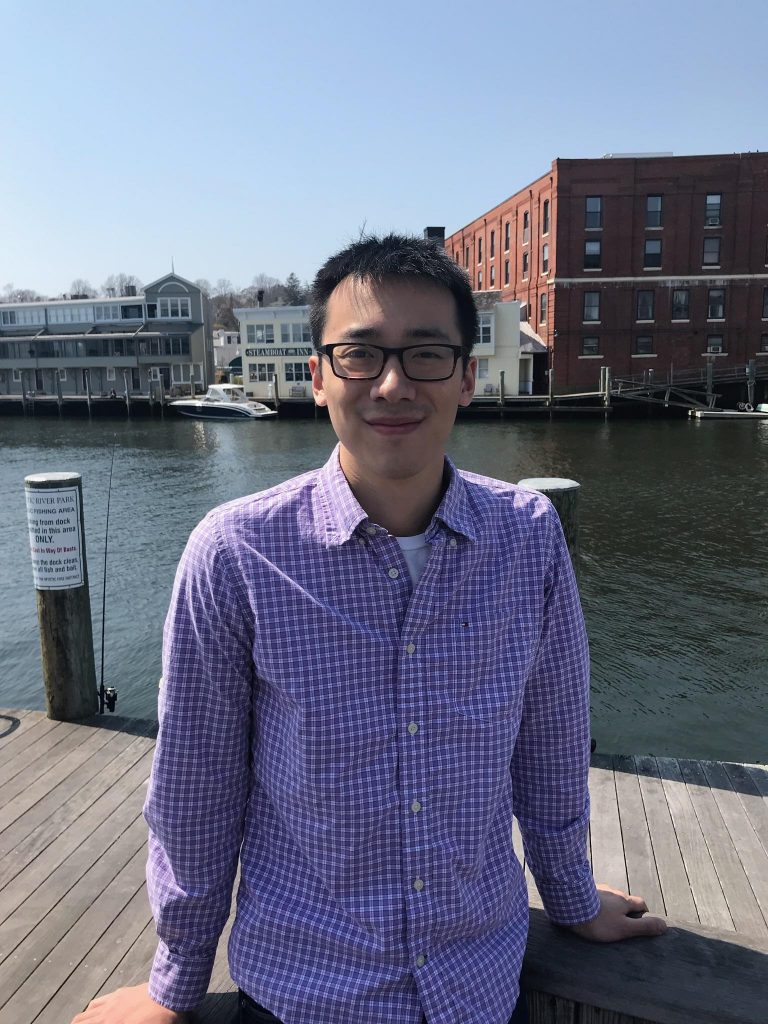
\includegraphics[width=0.70\textwidth]{images/chou.jpg}}
	\caption{Michael Chou}
	\end{subfigure} \quad\quad
	%
	\begin{subfigure}{0.25\textwidth}
	\captionsetup{labelformat=empty}
	\centering
	\fbox{
\includegraphics[width=0.90\textwidth]{images/daniels.jpeg}}
	\caption{Harris Daniels}
	\end{subfigure} \enskip
	%
	\begin{subfigure}{0.35\textwidth}
	\captionsetup{labelformat=empty}
	\centering
	\fbox{
\includegraphics[width=0.50\textwidth]{images/jimenez.png}}
	\caption{Enrique Gonz\'alez-Jim\'enez}
	\end{subfigure} \\
	%
	\begin{subfigure}{0.35\textwidth}
	\captionsetup{labelformat=empty}
	\centering
	\fbox{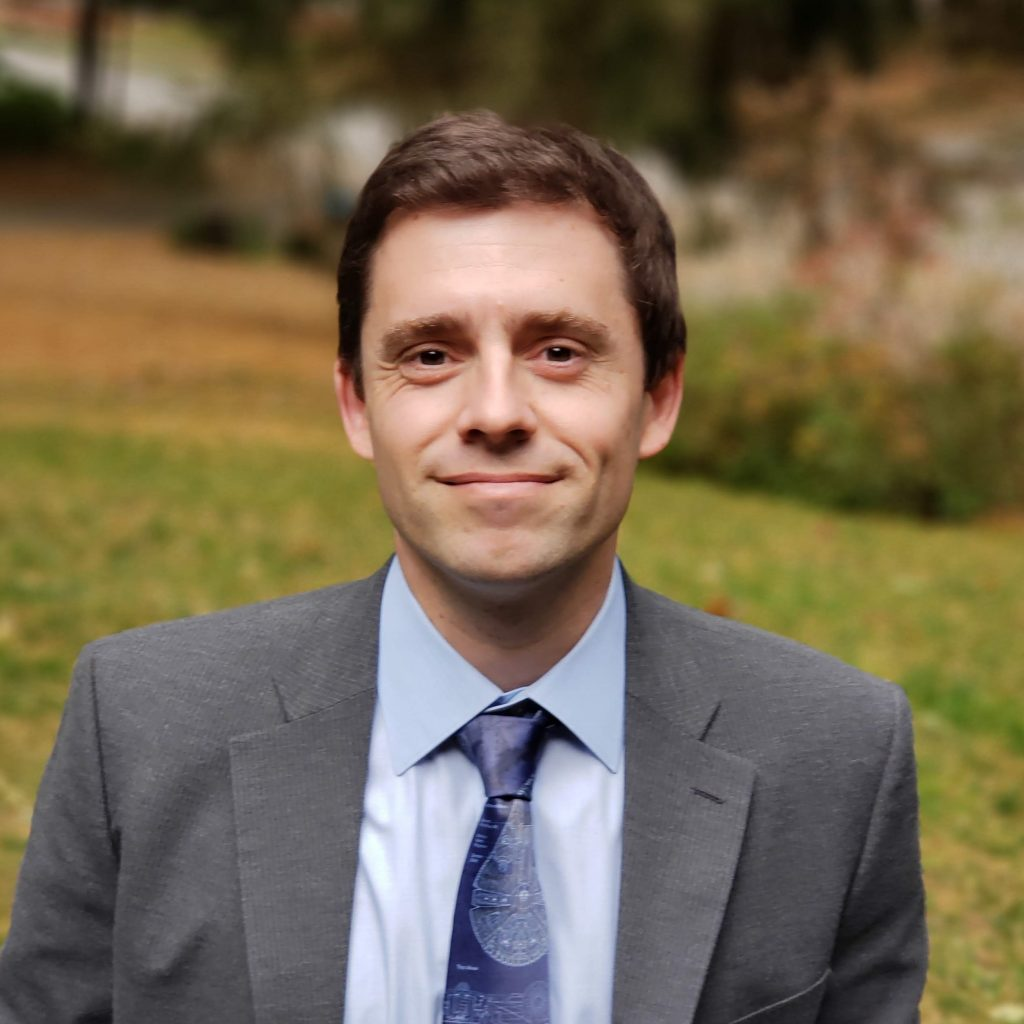
\includegraphics[width=0.6\textwidth]{images/robledo.jpg}}
	\caption{\'Alvaro Lozano-Robledo}
	\end{subfigure} \quad
	%
	\begin{subfigure}{0.25\textwidth}
	\captionsetup{labelformat=empty}
	\centering
	\fbox{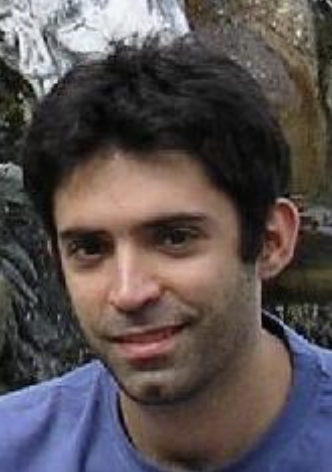
\includegraphics[width=0.62\textwidth]{images/najman2.png}}
	\caption{Filip Najman}
	\end{subfigure} \quad\quad
	%
	\begin{subfigure}{0.25\textwidth}
	\captionsetup{labelformat=empty}
	\centering
	\fbox{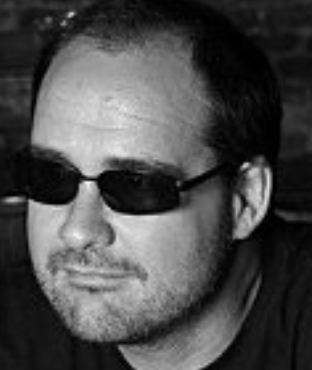
\includegraphics[width=0.75\textwidth]{images/tornero.png}}
	\caption{Jos\'e Tornero}
	\end{subfigure}
	\end{figure}
\end{frame}


% Cubic
\begin{frame}[plain]
\begin{thm}[Najman, 2012]
Let $K/\Q$ be a cubic number field and $E/\Q$ be a rational elliptic curve. Then
	\[
	E(F)_\tors \cong
	\begin{cases}
	\Z/n\Z, & n= 1,\ldots,10,12,13,14,18,21 \\
	\Z/2\Z \oplus \Z/2n\Z, & n= 1,\ldots,4,7
	\end{cases}
	\]
Moreover, the elliptic curve 162B1 over $\Q(\zeta_9)^+$ is the unique rational elliptic curve over a cubic number field with torsion subgroup $\Z/21\Z$.
\end{thm}
	\begin{figure}
	\captionsetup{labelformat=empty}
	\centering
	\fbox{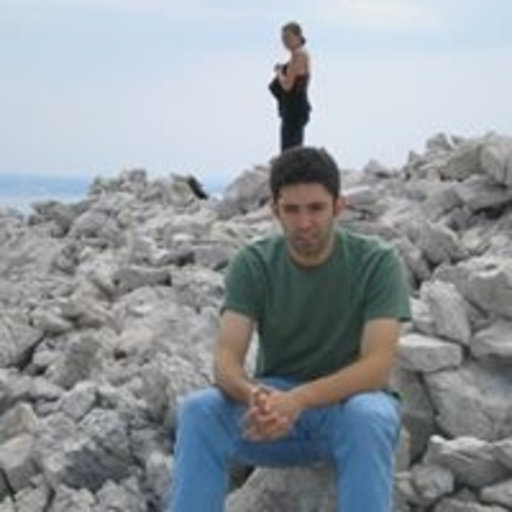
\includegraphics[width=0.30\textwidth]{images/najman.jpg}}
	\caption{\hspace{0.1cm}Filip Najman}
	\end{figure}
\end{frame}


% Chou
\begin{frame}[plain]
\begin{thm}[Chou, 2015]
Let $K/\Q$ be a quartic Galois field and $E/\Q$ be an elliptic curve. Then $E(K)_\tors$ is isomorphic to one of the following:
	\[
	\begin{cases}
	\Z/n\Z, & n= 1,\ldots,10,12,13,15,16 \\
	\Z/2\Z \oplus \Z/2n\Z, & n= 1,\ldots,6,8 \\
	\Z/3\Z \oplus \Z/3n\Z, & n= 1,2 \\
	\Z/4\Z \oplus \Z/4n\Z, & n= 1,2 \\
	\Z/5\Z \oplus \Z/5\Z \\
	\Z/6\Z \oplus \Z/6\Z
	\end{cases}
	\]
\end{thm}
	\begin{figure}
	\captionsetup{labelformat=empty}
	\centering
	\fbox{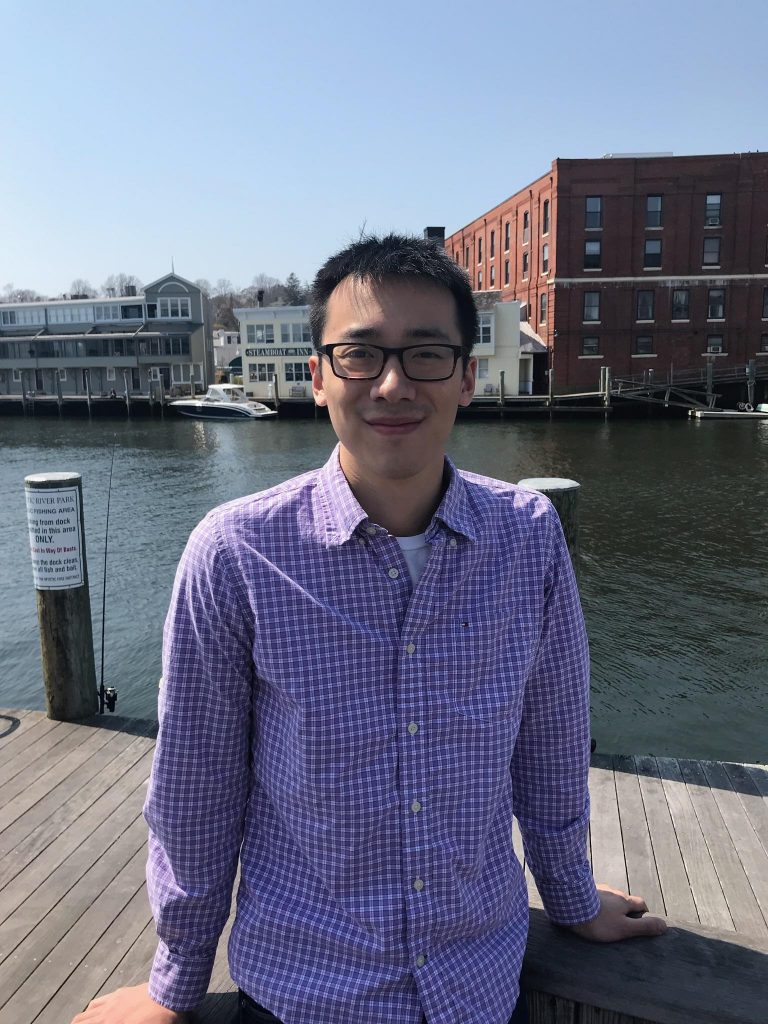
\includegraphics[width=0.18\textwidth]{images/chou.jpg}}
	\caption{Michael Chou}
	\end{figure}
\end{frame}


% M.
\begin{frame}[plain]
\begin{thm}[M.]
Let $K/\Q$ be a nonic Galois field and $E/\Q$ be an elliptic curve. Then $E(K)_\tors$ is isomorphic to one of the following groups:
	\[
	\begin{cases}
	\Z/n\Z, & n= 1,2,\ldots,10,12,13,\ldots,16,18,19,21,25,27  \\
	\Z/2\Z \oplus \Z/2n\Z, & n= 1,\ldots,7,9
	\end{cases}
	\]
\end{thm}
	\begin{figure}
	\captionsetup{labelformat=empty}
	\centering
	\fbox{\includegraphics[width=0.25\textwidth]{images/mcwhorter.png}}
	\caption{Caleb McWhorter}
	\end{figure}
\end{frame}


% S_Q(d)
\begin{frame}[plain]
	\begin{thm}[Mazur, Parent, Derickx, Kammienny, Stein, Stoll, Lozano-Robledo, et al.]
		\[
		\begin{split}
		S_\Q(\{1,2\})&= \{ 2,3,5,7 \} \\
		S_\Q(\{3,4\})&= \{ 2,3,5,7,13 \} \\
		S_\Q(\{5,6,7\})&= \{ 2,3,5,7,11,13 \} \\
		S_\Q(8)&= \{ 2,3,5,7,11,13 \} \\
		S_\Q(\{9,10,11\})&= \{ 2,3,5,7,11,13,17,19 \} \\
		S_\Q(\{12,\ldots,20\})&= \{2,3,5,7,11,13,17,19,37 \} \\
		S_\Q(21)&= \{ 2,3,5,7,11,13,17,19,37,43 \}
		\end{split}
		\]
	\end{thm}
\end{frame}


% Serre
\begin{frame}[plain]
\begin{rem}
Lozano-Robledo computes $S_\Q(d)$ for $1 \leq d \leq 21$, and gives a conjecturally formula valid for all $1 \leq d \leq 42$, following from a positive answer to Serre's uniformity question.
\end{rem}
	\begin{figure}[h]
	\centering
	\begin{subfigure}{\textwidth}
	\captionsetup{labelformat=empty}
	\centering
	\fbox{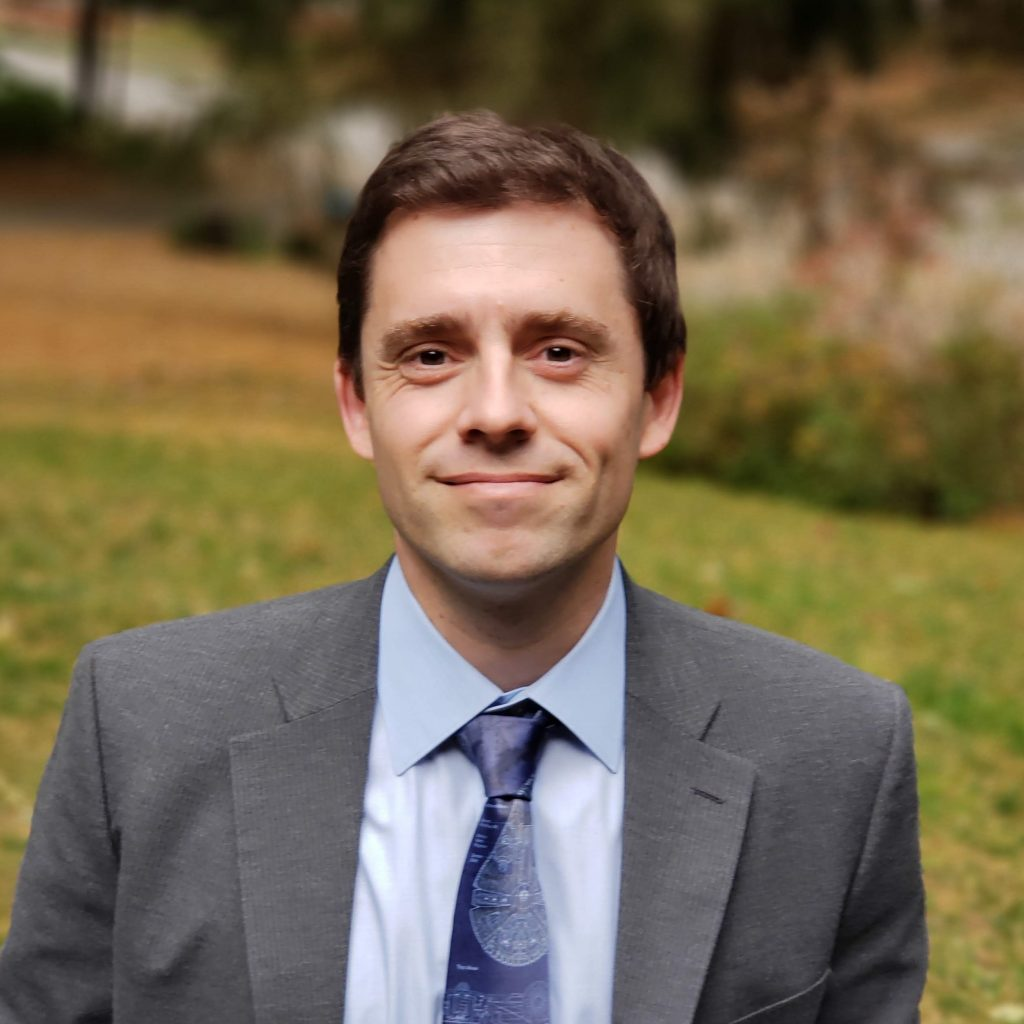
\includegraphics[width=0.25\textwidth]{images/robledo.jpg}}
	\caption{\'Alvaro Lozano-Robledo}
	\end{subfigure}
	\end{figure}
\begin{rem}
Furthermore, Enrique Gonz\'alez-Jim\'enez and Filip Najman determine all possible prime orders of a point $P \in E(K)_\tors$, where $[K : \Q]= d$ for all $d \leq 3\,342\,296$.
\end{rem}
\end{frame}


% Min Field
\begin{frame}[plain]
\begin{thm}[Gonz\'alez-Jim\'enez, Lozano-Robledo, 2015]
Let $E/\Q$ be an elliptic curve without CM. Let $1 \leq s \leq N$ be fixed integers, and let $T \subseteq E[2^N]$ be a subgroup isomorphic to $\Z/2^s/Z \oplus \Z/2^N \Z$. Then $[\Q(T) \colon \Q]$ is divisible by 2 if $s=N=2$, and otherwise by $2^{2N+2s-8}$ if $N \geq 3$, unless $s \geq 4$ and $j(E)$ is one of the two values:
	\[
	- \dfrac{3 \cdot 18249920^3}{17^{16}}\; \text{ or } - \dfrac{7 \cdot 1723187806080^3}{79^{16}}
	\]
in which case $[\Q(T) \colon \Q]$ is divisible by $3 \cdot 2^{2N+2s-9}$. Moreover, this is best possible in that there are one-parameter families $E_{s,N}(t)$ of elliptic curves over $\Q$ such that for each $s, N \geq 0$ and each $t \in \Q$, and subgroups $T_{s,N} \in E_{s,N}(t)(\ov{\Q})$ isomorphic to $\Z/2^s\Z \oplus \Z/2^N\Z$ such that $[\Q(T_{s,N}) \colon \Q]$ is equal to the bound given above. 
\end{thm}
\end{frame}


% Inf. Extensions
\begin{frame}[plain]
\ctext{What about infinite extensions?}
\end{frame}


% 2-abelian
\begin{frame}[plain]
\begin{thm}[Laska, Lorenz, 1985; Fujita, 2005]
Let $E/\Q$ be an elliptic curve. The torsion subgroup $E(\Q(2^\infty))_\tors$ is finite and is isomorphic to precisely one of the following:
	\[
	\begin{cases}
	\Z/n\Z, & n=1,3,5,7,9,15 \\
	\Z/2\Z \oplus \Z/2n\Z, & n= 1,\ldots,6,8 \\
	\Z/3\Z \oplus \Z/3\Z \\
	\Z/4\Z \oplus \Z/4n\Z, & n= 1,\ldots,4 \\
	\Z/2n\Z \oplus \Z/2n\Z, & n= 3,4
	\end{cases}
	\]
\end{thm}
	\begin{figure}[h]
	\centering
	\begin{subfigure}{0.3\textwidth}
	\captionsetup{labelformat=empty}
	\centering
	\fbox{
\includegraphics[width=0.72\textwidth]{images/laska.png}}
	\caption{Michael Laska}
	\end{subfigure}
	%
	\begin{subfigure}{0.3\textwidth}
	\captionsetup{labelformat=empty}
	\centering
	\fbox{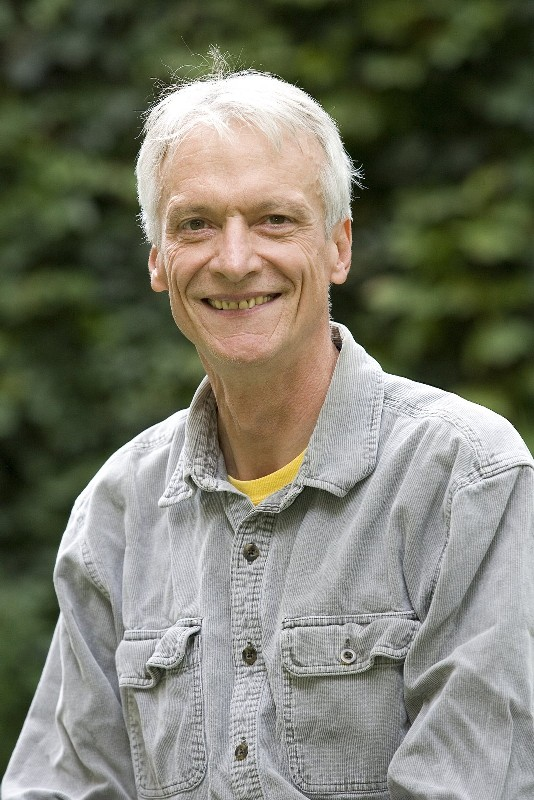
\includegraphics[width=0.87\textwidth]{images/lorenz.jpeg}}
	\caption{Martin Lorenz}
	\end{subfigure}
	%
	\begin{subfigure}{0.3\textwidth}
	\captionsetup{labelformat=empty}
	\centering
	\fbox{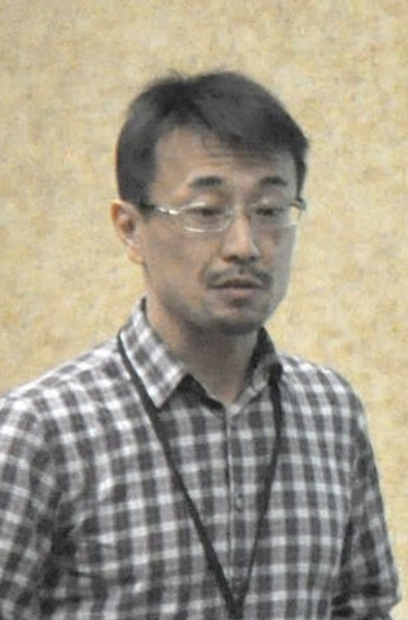
\includegraphics[width=0.8\textwidth]{images/fujita.png}}
	\caption{Yasutsugu Fujita}
	\end{subfigure}
	\end{figure}
\end{frame}


% 3-abelian
\begin{frame}[plain]
\begin{thm}[Daniels, Lozano-Robledo, Najman, Sutherland, 2017]
Let $E/\Q$ be an elliptic curve. Then $E(\Q(3^\infty))_\tors$ is finite and is isomorphic to precisely one of the following:
	\[
	\begin{cases}
	\Z/2\Z \oplus \Z/2n\Z, & n= 1,2,4,5,7,8,13 \\
	\Z/4\Z \oplus \Z/4n\Z, & n= 1,2,4,7 \\
	\Z/6\Z \oplus \Z/6n\Z, &  n= 1,2,3,5,7 \\
	\Z/2n\Z \oplus \Z/2n\Z, & n= 4,6,7,9
	\end{cases}
	\]
All but four of the possibilities occur infinitely often: $(4,28)$, $(6,30)$, $(6,42)$, $(14,14)$, which occur for only 2, 2, 4, and 1 elliptic curves, respectively. 
\end{thm}
	\begin{figure}[h]
	\centering
	\begin{subfigure}{0.15\textwidth}
	\captionsetup{labelformat=empty}
	\centering
	\fbox{
\includegraphics[width=1.05\textwidth]{images/daniels.jpeg}}
	\caption{\tiny{Harris Daniels}}
	\end{subfigure}
	%
	\begin{subfigure}{0.25\textwidth}
	\captionsetup{labelformat=empty}
	\centering
	\fbox{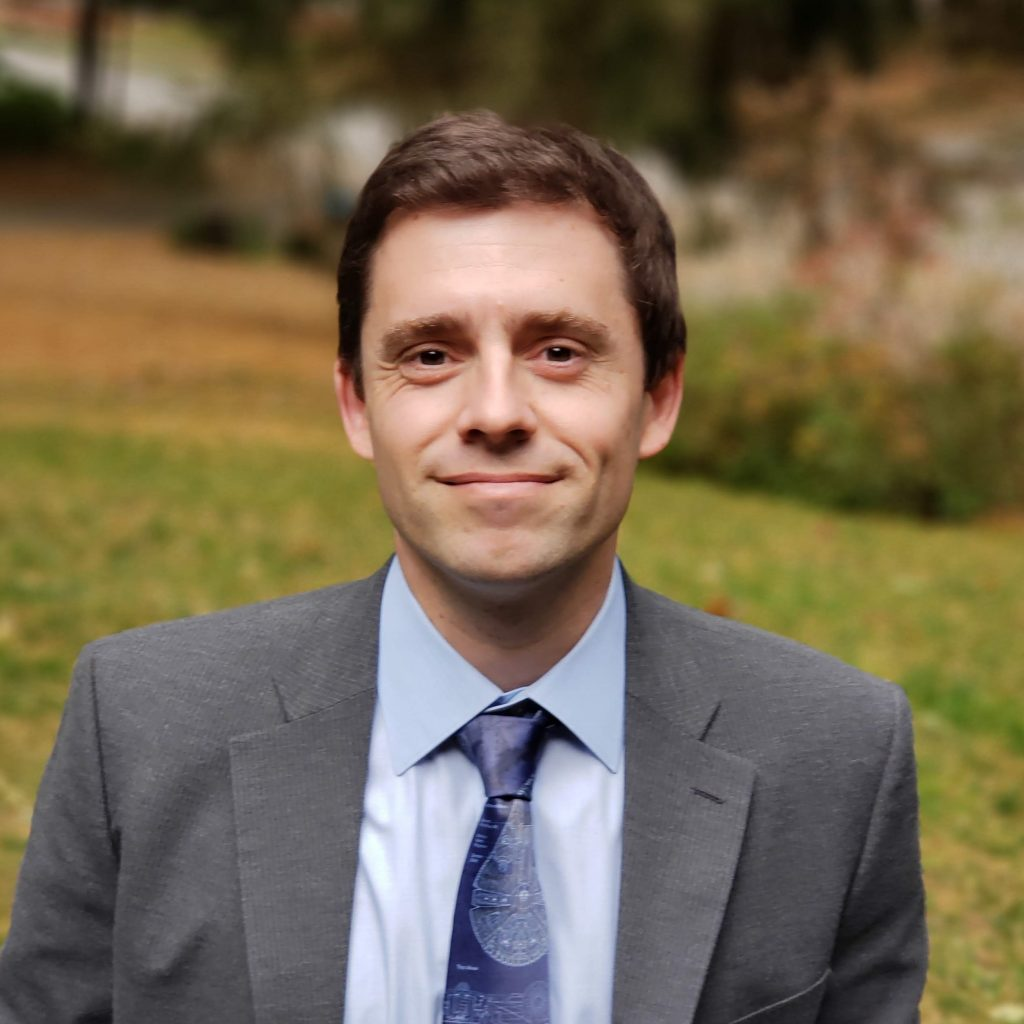
\includegraphics[width=0.65\textwidth]{images/robledo.jpg}}
	\caption{\tiny{\'Alvaro Lozano-Robledo}}
	\end{subfigure}
	%
	\begin{subfigure}{0.15\textwidth}
	\captionsetup{labelformat=empty}
	\centering
	\fbox{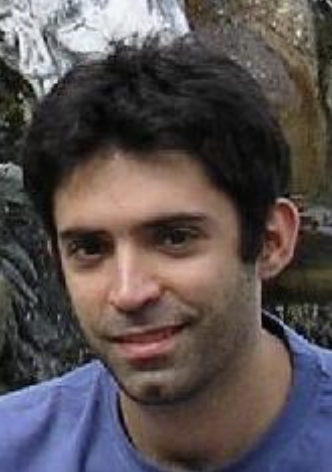
\includegraphics[width=0.75\textwidth]{images/najman2.png}}
	\caption{\tiny{Filip Najman}}
	\end{subfigure}
	%
	\begin{subfigure}{0.15\textwidth}
	\captionsetup{labelformat=empty}
	\centering
	\fbox{\includegraphics[width=0.98\textwidth]{images/sutherland.jpg}}
	\caption{\tiny{Drew Sutherland}}
	\end{subfigure}
	\end{figure}
\end{frame}


% Other Options
\begin{frame}[plain]
\ctext{What about other types of fields?}
\end{frame}


% McDonald
\begin{frame}[plain]
\begin{thm}[McDonald, 2017]
Let $K= \F_q(T)$, where $q=p^n$. Let $E/K$ be non-isotrivial. If $p \nmid E(K)_\tors$, then $E(K)_\tors$ is one of the following: $0,\Z/2\Z, \ldots,\Z/10\Z,\Z/12\Z, \Z/2\Z \oplus \Z/2\Z, \Z/2\Z \oplus \Z/4\Z, \Z/2\Z \oplus \Z/6\Z, \Z/2\Z \oplus \Z/8\Z, \Z/3\Z \oplus \Z/3\Z, \Z/3\Z \oplus \Z/6\Z, \Z/4\Z \oplus \Z/4\Z, \Z/5\Z \oplus \Z/5\Z$.

If $p \mid \#E(K)_\tors$, then $p \leq 11$, and $E(K)_\tors$ is one of
	\[
	\begin{cases}
	\Z/p\Z, & p=2,3,5,7,11 \\
	\Z/2p\Z, & p=2,3,5,7 \\
	\Z/3p\Z, & p=2,3,5 \\
	\Z/4p\Z, & p=2,3 \\
	\Z/5p\Z, & p=2,3 \\
	\Z/5\Z \oplus \Z/10\Z, & p=2 \\
	\Z/2\Z \oplus \Z/12\Z, & p=3 \\
	\Z/2\Z \oplus \Z/10\Z, & p=5
	\end{cases}
	\]
\end{thm}
\end{frame}


% McDonald
\begin{frame}[plain]
\ctext{
	\begin{figure}
	\captionsetup{labelformat=empty}
	\centering
	\fbox{\includegraphics[width=0.30\textwidth]{images/mcdonald.jpg}}
	\caption{Robert McDonald}
	\end{figure}
}
\end{frame}




% Other Questions
\begin{frame}[plain]
\ctext{What are other questions one might ask?}
\end{frame}


% Bounded
\begin{frame}[plain]
\ctext{How large can the torsion be?}
\end{frame}


% Bounded 2
\begin{frame}[plain]
\begin{thm}[Merel,1996]
Let $K$ be a number field of degree $[K:\Q]=d>1$. There is a number $B(d)>0$ such that $|E(K)_\tors| \leq B(d)$ for all elliptic curves $E/K$.
\end{thm}
	\begin{figure}
	\captionsetup{labelformat=empty}
	\centering
	\fbox{\includegraphics[width=0.50\textwidth]{images/merel.jpg}}
	\caption{Lo\"ic Merel}
	\end{figure}
\end{frame}


% Conj
\begin{frame}[plain]
\begin{conj}[Clark, Cook, Stakewicz]
There is a constant $C$ such that $B(d) \leq C\, d \log\log d$ for all $d \geq 3$.
\end{conj}
	\begin{figure}[h]
	\centering
	\begin{subfigure}{0.3\textwidth}
	\captionsetup{labelformat=empty}
	\centering
	\fbox{\includegraphics[width=0.70\textwidth]{images/clark.jpg}}
	\caption{Pete Clark}
	\end{subfigure} \quad
	%
	\begin{subfigure}{0.3\textwidth}
	\captionsetup{labelformat=empty}
	\centering
	\fbox{\includegraphics[width=0.82\textwidth]{images/cook.png}}
	\caption{Brian Cook}
	\end{subfigure}
	%
	\begin{subfigure}{0.3\textwidth}
	\captionsetup{labelformat=empty}
	\centering
	\fbox{\includegraphics[width=0.65\textwidth]{images/stankewicz.png}}
	\caption{James Stankewicz}
	\end{subfigure}
	\end{figure}
\end{frame}


% Silverman
\begin{frame}[plain]
\begin{thm}[Hindry, Silverman, 1999]
Let $K$ be a field of degree $d \geq 2$ and $E/K$ be an elliptic curve such that $j(E)$ is an algebraic integer. Then we have
	\[
	|E(K)_\tors| \leq 1\,977\,404 \cdot d \log d
	\]
\end{thm}
	\begin{figure}[h]
	\centering
	\begin{subfigure}{0.3\textwidth}
	\captionsetup{labelformat=empty}
	\centering
	\fbox{\includegraphics[width=1.0\textwidth]{images/hindry.jpeg}}
	\caption{Marc Hindry}
	\end{subfigure}
	%
	\begin{subfigure}{0.3\textwidth}
	\captionsetup{labelformat=empty}
	\centering
	\fbox{\includegraphics[width=0.77\textwidth]{images/silverman.jpg}}
	\caption{Joseph Silverman}
	\end{subfigure}
	\end{figure}
\end{frame}


% Clark, Pollack
\begin{frame}[plain]
\begin{thm}[Clark, Pollack, 2015]
There is an absolute, effective constant $C$ such that for all number fields $K$ of degree $d \geq 3$ and all elliptic curves $E/K$ with CM, we have $|E(K)_\tors| \leq C\, d \log \log d$.
\end{thm}
	\begin{figure}[h]
	\centering
	\begin{subfigure}{0.3\textwidth}
	\captionsetup{labelformat=empty}
	\centering
	\fbox{\includegraphics[width=0.62\textwidth]{images/clark2.png}}
	\caption{Pete Clark}
	\end{subfigure}
	%
	\begin{subfigure}{0.3\textwidth}
	\captionsetup{labelformat=empty}
	\centering
	\fbox{\includegraphics[width=0.90\textwidth]{images/pollack.jpg}}
	\caption{Paul Pollack}
	\end{subfigure}
	\end{figure}
\end{frame}


% Prime Point
\begin{frame}[plain]
\begin{thm}[Merel, 1996]
Let $F/\Q$ be a number field of degree $d$. If $P \in E(F)$ is a point of exact prime power $p^n$, then $p \leq 3^{3d^2}$.
\end{thm} 
	\begin{figure}[h]
	\centering
	\begin{subfigure}{0.3\textwidth}
	\captionsetup{labelformat=empty}
	\centering
	\fbox{\includegraphics[width=0.90\textwidth]{images/merel.jpg}}
	\caption{Lo\"ic Merel}
	\end{subfigure}
	%
	\begin{subfigure}{0.3\textwidth}
	\captionsetup{labelformat=empty}
	\centering
	\fbox{\includegraphics[width=0.95\textwidth]{images/parent.png}}
	\caption{Pierre Parent}
	\end{subfigure}
	\end{figure}
\begin{rem}
In 1999, Parent improved this to $p^n \leq 129(5^d - 1)(3d)^6$.
\end{rem}
\end{frame}


% Lozano Prime
\begin{frame}[plain]
\begin{thm}[Lozano-Robledo, 2013]
Let $K/\Q$ be a number field of degree $d$ and suppose there is an elliptic curve $E/K$ with CM by a full order with a point of order $p^n$, then
	\[
	\varphi(p^n) \leq 24\, e_{\max}(p,K/\Q) \leq 24\, d
	\]
\end{thm}
	\begin{figure}[h]
	\centering
	\begin{subfigure}{\textwidth}
	\captionsetup{labelformat=empty}
	\centering
	\fbox{\includegraphics[width=0.25\textwidth]{images/robledo.jpg}}
	\caption{\'Alvaro Lozano-Robledo}
	\end{subfigure}
	\end{figure}
\end{frame}


% Other
\begin{frame}[plain]
\ctext{What are even more questions one can consider?}
\end{frame}


% Other
\begin{frame}[plain]
\ctext{Over what fields do torsion subgroups occur?}
\ctext{What happens over other intermediate extensions?}
\ctext{What about other fields?}
\ctext{How `common' are given torsion subgroups?}
\end{frame}


% Other
\begin{frame}[plain]
\ctext{What all this means is the number of interesting questions about torsion subgroups of elliptic curves is unbounded\dots unlike the rank\dots probably.}
\end{frame}


% Questions
\begingroup
\setbeamercolor{background canvas}{bg= gray, fg=white}
\begin{frame}[plain]
\phantom{x} \vfill
\begin{center} {\huge \textcolor{white}{Questions?}} \end{center}
\vfill
\end{frame}
\endgroup